%für Sprache, A4 Blatt, float, Grafiken, UTF Codierung, PDF, Color, Seitenabstand, Listings
\documentclass[a4papr,12pt]{article}
\usepackage[utf8]{inputenc}
\usepackage[ngerman]{babel}
\usepackage{graphicx}
\usepackage{float}
\usepackage{textcomp}
\usepackage{pdfpages}
\usepackage{tikz}
\usepackage{hyperref}
\usepackage{geometry}
\usepackage{listings}
\usepackage{color}

%Mathematics
\usepackage{amstext}
\usepackage{amssymb}
\usepackage{amsmath}
\usepackage{amsfonts}
\usepackage{mathrsfs}
\usepackage{mathtools}

%Für Kopfzeile den Style
\usepackage{fancyhdr}
\pagestyle{fancy}
\lhead{ADE - Übung 2}
\rhead{Andreas Roither, \today{}}
\newcommand{\Cross}{\mathbin{\tikz [x=1.4ex,y=1.4ex,line width=.2ex] \draw (0,0) -- (1,1) (0,1) -- (1,0);}}%

%Seitenabstand A4 Blatt
\geometry{a4paper}
\geometry{top=25mm,bottom=25mm,left=23mm,right=20mm}

% macro to select a scaled-down version of Bera Mono (for instance)
\makeatletter
\newcommand\BeraMonottfamily{%
  \def\fvm@Scale{0.85}% scales the font down
  \fontfamily{fvm}\selectfont% selects the Bera Mono font
}
\makeatother

%Hyperref zum anklicken von Überschriften in Texmaker + Farben einstellen
\hypersetup{
	colorlinks,
	citecolor=black,
	filecolor=black,
	linkcolor=blue,
	urlcolor=black
}

\definecolor{mygreen}{rgb}{0,0.6,0}
\definecolor{mygray}{rgb}{0.5,0.5,0.5}
\definecolor{mymauve}{rgb}{0.58,0,0.82}

%Zum Pascal Code einfügen mit lstinputlisting[language=Pascal] {../blabla.pas}
\lstset{ %
  backgroundcolor=\color{white},   % choose the background color; you must add \usepackage{color} or 								  \usepackage{xcolor}
  basicstyle=\BeraMonottfamily,        % the size of the fonts that are used for the code
  breakatwhitespace=false,         % sets if automatic breaks should only happen at whitespace
  breaklines=true,                 % sets automatic line breaking
  captionpos=b,                    % sets the caption-position to bottom
  commentstyle=\color{mygreen},    % comment style
  deletekeywords={...},            % if you want to delete keywords from the given language
  escapeinside={\%*}{*)},          % if you want to add LaTeX within your code
  extendedchars=true,              % lets you use non-ASCII characters; for 8-bits encodings only, 												does not work with UTF-8
  frame=single,	               % adds a frame around the code
  keepspaces=true,                 % keeps spaces in text, useful for keeping indentation of code 									  (possibly needs columns=flexible)
  keywordstyle=\color{blue},       % keyword style
  language=Octave,                 % the language of the code
  otherkeywords={...},           % if you want to add more keywords to the set
  numbers=left,                    % where to put the line-numbers; possible values are (none, left, 								  right)
  numbersep=5pt,                   % how far the line-numbers are from the code
  numberstyle=\tiny\color{black}, % the style that is used for the line-numbers
  rulecolor=\color{black},         % if not set, the frame-color may be changed on line-breaks within 								  not-black text (e.g. comments (green here))
  showspaces=false,                % show spaces everywhere adding particular underscores; it 														overrides 'showstringspaces'
  showstringspaces=false,          % underline spaces within strings only
  showtabs=false,                  % show tabs within strings adding particular underscores
  stepnumber=2,                    % the step between two line-numbers. If it's 1, each line will be 								  numbered
  stringstyle=\color{mymauve},     % string literal style
  title=\getlstname,
  tabsize=2,	                    % sets default tabsize to 2 spaces
  inputencoding=latin1,
  columns=fullflexible
}

\lstset{literate=%
	{Ö}{{\"O}}1
	{Ä}{{\"A}}1
	{Ü}{{\"U}}1
	{ß}{{\ss}}1
	{ü}{{\"u}}1
	{ä}{{\"a}}1
	{ö}{{\"o}}1
	{~}{{\textasciitilde}}1
}

%Filenamen und Pfad trennen
\makeatletter
\DeclareRobustCommand{\getlstname}{%
\begingroup
  % \lstname seems to change hyphens into \textendash
  \def\textendash{-}%
  \filename@parse{\lstname}%
  \texttt{\filename@base.\filename@ext}%
\endgroup
}


\begin{document}

%ANGABE 
\thispagestyle{plain}
\includepdf[pagecommand={     
\begin{tikzpicture}[remember picture, overlay]\node at (15.8, -1.35) {3 h};\end{tikzpicture}
\begin{tikzpicture}[remember picture, overlay]\node at (7.6, -1.35) {Andreas Roither};\end{tikzpicture}
\begin{Huge}
\begin{tikzpicture}[remember picture, overlay]\node at (-1, -1.9) {X};\end{tikzpicture}
\end{Huge}
}]{Angabe/Uebung02.pdf}
%\includepdf[pages=2-]{Angabe/Uebung 2.pdf}

\section*{Übung 2}
\subsection*{Aufgabe 1}

\lstinputlisting[language=Pascal] {../spannweite.pas}
\begin{figure}[H]
	\centering
	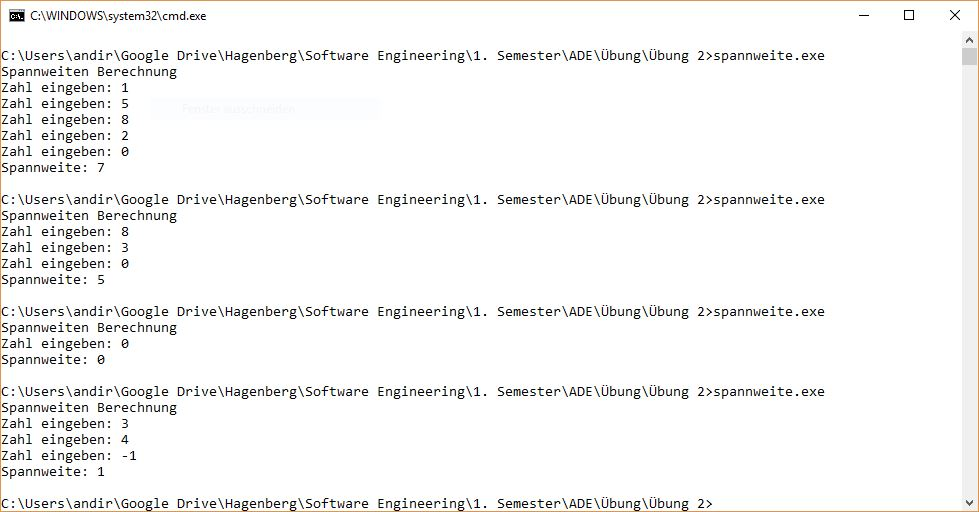
\includegraphics[scale=0.653]{./pictures/spannweite.png}
	\caption{Testfälle Spannweitenberechnung}
	\label{fig: Spannweiten Berechnung}
\end{figure}

\section*{Testfälle}
Bei der Spannweitenberechnung wurden 4 mögliche Testfälle ausprobiert.
Die Reihenfolge der Zahlen, negative Zahlen und Nulleingaben wurden berücksichtigt und getestet.
\newpage

\subsection*{Aufgabe 2}

\lstinputlisting[language=Pascal] {../sortieren.pas}
\begin{figure}[H]
	\centering
	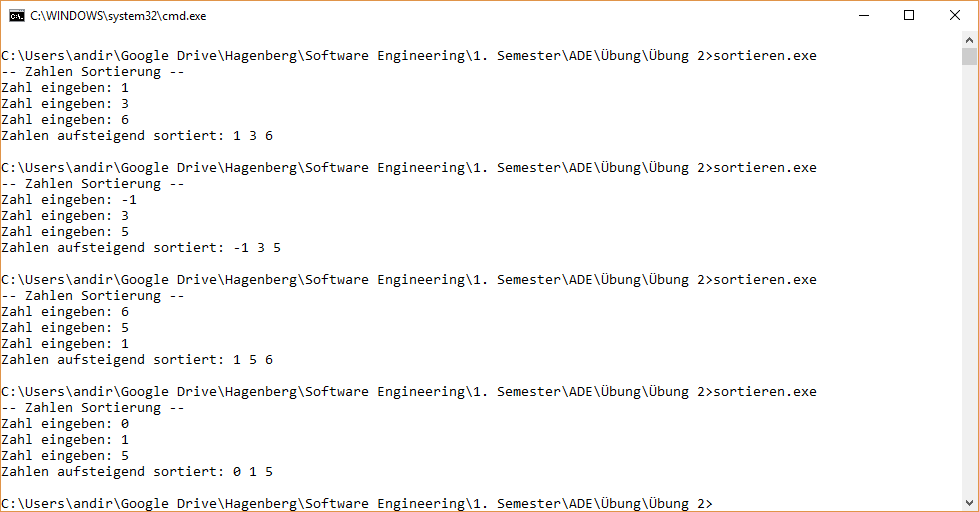
\includegraphics[scale=0.653]{./pictures/sortieren.png}
	\caption{Testfälle Sortieralgorithmus}
	\label{fig: Sortieralgorithmus}
\end{figure}

\section*{Testfälle}
Für den Sortieralgorithmus wurde die Reihenfolge der Zahlen, negative Zahlen, und Nulleingabe getestet.

\newpage

\subsection*{Aufgabe 3}
\subsubsection*{Lösungsidee}
Bei der Quadratwurzelberechnung soll mithilfe einer Reellen Zahl und einer Fehlerschranke die Quadratische Wurzel der Reellen Zahl berechnet werden. Dazu muss die Richtigkeit der Eingabe überprüft werden und entsprechende Fehlermeldungen ausgegeben werden. Nach der Überprüfung der Eingabe soll mithilfe der Newtonsche Iterationsformel eine Näherung für $y \approx \sqrt{x}$ berechnet werden. Mithilfe der Formel $ y1 = \frac{1}{2}(y0 + \frac{x}{y_{0}})$ und einer Repeat Until Schleife die nach 50 Iterationen abbricht wird eine Näherung für die Eingabe berechnet.

\lstinputlisting[language=Pascal] {../quadratwurzel.pas}
\begin{figure}[H]
	\centering
	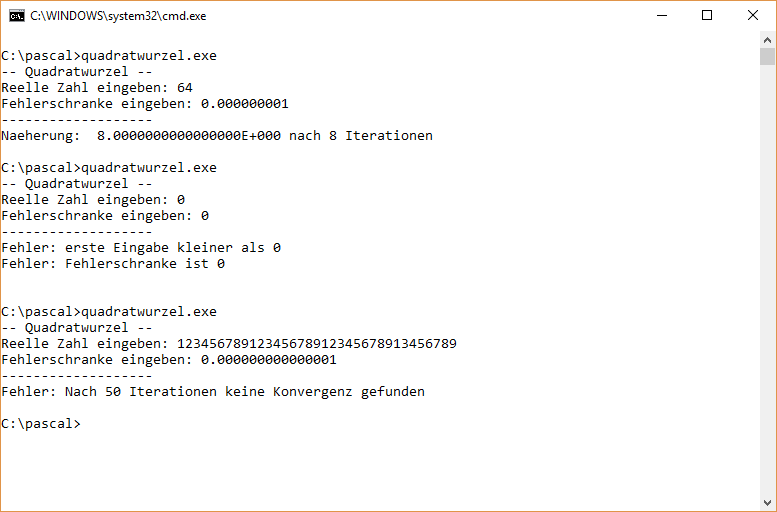
\includegraphics[scale=0.75]{./pictures/quadratwurzel.png}
	\caption{Testfälle Quadratwurzelberechnung}
	\label{fig: label}
\end{figure}

\section*{Testfälle}
Bei der Quadratwurzelberechnung wurde auf verschiedene Fehlerquellen getestet.
Der erste Testfall dient zur generellen Überprüfung der Berechnung, der zweite Testfall dient zur Überprüfung der Eingabe. Der dritte Testfall soll zeigen das nach 50 Iterationen abgebrochen wird.

\newpage
\end{document}





